\documentclass{beamer} 
%\documentclass[handout]{beamer} 
\usetheme{Ilmenau}
\usepackage{graphicx,verbatim,hyperref}
\usepackage{textpos}

\usecolortheme{beaver}
\useinnertheme{default}
\setbeamertemplate{itemize item}[triangle]
\setbeamertemplate{itemize subitem}[triangle]
\setbeamertemplate{itemize subsubitem}[circle]
\setbeamertemplate{enumerate items}[default]
\setbeamertemplate{blocks}[upper=block head,rounded]
\setbeamercolor{item}{fg=black}
\usefonttheme{serif} %should allow ccfonts to take effect

\usepackage{cite}
\usepackage{times, verbatim,xcolor,bm}
%\usepackage[usenames,dvipsnames]{color}
\usepackage{amsbsy,amssymb, amsmath, amsthm}
\usepackage{booktabs}
%David miller's fonts
	\usepackage[T1]{fontenc}
	\usepackage[boldsans]{ccfonts}
	%\usepackage[boldsans]{concmath}
	\usepackage[euler-hat-accent]{eulervm}

\newcommand{\al}{\alpha}
\newcommand{\expect}{\mathbb{E}}
\newcommand{\Bt}{B(\bm{\tau^a})}
\newcommand{\bta}{\bm{\tau^a}}
\newcommand{\btn}{\bm{\tau^{tw}}}
\newcommand{\ga}{\gamma}
\newcommand{\ve}{\varepsilon}
\newcommand{\ta}{\theta}
\newcommand{\de}{\delta}
\newcommand{\ov}{\overline}
\newcommand{\un}{\underline}

\newenvironment{changemargin}[2]{% 
  \begin{list}{}{% 
    \setlength{\topsep}{0pt}% 
    \setlength{\leftmargin}{#1}% 
    \setlength{\rightmargin}{#2}% 
    \setlength{\listparindent}{\parindent}% 
    \setlength{\itemindent}{\parindent}% 
    \setlength{\parsep}{\parskip}% 
  }% 
  \item[]}{\end{list}} 
	
	\let\Tiny=\tiny

%\usepackage{appendixnumberbeamer}


\title[Endogenous Politics and the Design of Trade Institutions\hspace{2.05in}\insertframenumber/\inserttotalframenumber]{Endogenous Politics and \\ the Design of Trade Institutions}
%\author[Kristy Buzard]{Kristy Buzard \\ Syracuse University and The Wallis Institute \\ kbuzard@syr.edu}
\author[Kristy Buzard]{\texorpdfstring{Kristy Buzard\newline Syracuse University \newline\url{kbuzard@syr.edu}}{Kristy Buzard}}
\date{March 2, 2018}
\begin{document}
\maketitle
%\insertpresentationendpage removed b/c of appendix




\section{Overview}
\subsection{Preview}
\begin{frame}{The Questions}

\pause
\begin{enumerate}[<+->]
\item Can trade agreements (TAs) be used to manipulate domestic lobbying incentives?
	\begin{itemize}
		\item Government objective function
	\end{itemize}
\vskip.1in
	\item What is the optimal design of various trade agreement properties?
	\begin{itemize}
		\item Exogenous vs. endogenous politics
	\end{itemize}
\end{enumerate}

\end{frame}


\begin{frame}{Preview}
\frametitle{Political Economy of Trade Institutions}
\pause
With a few exceptions, TA design literature has taken political economy forces to be exogenous. I:
\pause
\begin{itemize}[<+->]
	\item endogenize politics into a standard model for studying TA design questions
		\begin{itemize}
			\item use this to examine gov't objective
		\end{itemize}
	\item carefully distinguish between dynamics induced by exogenous and endogenous politics for
		\begin{itemize}[<+->]
			\item base case with tariff caps
			\item tariff caps with escape clause
		\end{itemize}
	\item examine escape clause design when both exogenous and endogenous forces are present
\end{itemize}
\end{frame}


\begin{frame}{Preview}
\frametitle{Results}

\pause
\begin{itemize}[<+->]
	\item TAs may be used to manipulate domestic political actors (even with no long-run distortions)
	\item Simple modeling framework can capture results from models of both exogenous and endogenous politics
		\begin{itemize}
			\item For both tariff caps and escape clauses, endogenous politics changes outcomes dramatically
		\end{itemize}
	\item Standard, theoretical escape clause can't work in the presence of endogenous political pressure
		\begin{itemize}
			\item Points to real-world design of WTO Agreement on Safeguards
			\item May explain why escape clause has fallen out of use
		\end{itemize}
\end{itemize}
\end{frame}

\begin{comment}
\begin{frame}{Outline of Talk}
\pause
\begin{enumerate}[<+->]
	\item Model
	\item Government Objective Function
	\item Base Model with Tariff Caps
	\item Escape Clause
	\item Conclusion
\end{enumerate}
\end{frame}
\end{comment}








\section{Model}
\subsection{Economic and Political Structure}
\begin{frame}{Economy}
Two countries: home and foreign (${}^*$)
\pause
\begin{itemize}[<+->]
	\item Separable in two goods: $X$ and $Y$
			\begin{itemize}
				\item $P_i$: home price of good $i$
				\item $P_i^*$: foreign price of good $i$
			\end{itemize}
	\item Demand identical for both goods in both countries
		\begin{itemize}
			\item $D(P_i) = 1 - P_i$
		\end{itemize}
	\item Supply: $Q_X^*(P_X) > Q_X(P_X)$ $\forall P_X$; symmetric for $Y$ 
		\begin{itemize}
			\item $Q_X(P_X) = \frac{P_X}{2}$; $Q_Y(P_Y) = P_Y$
			\item Home net importer of $X$, net exporter of $Y$
		\end{itemize}
\end{itemize}

\end{frame}

\begin{frame}{Policy and Politics}

\pause
Home levies $\tau$ on $X$, Foreign levies $\tau^*$ on $Y$
\pause
\begin{itemize}
	\item $P_X=P_X^W + \tau$ increasing in $\tau$
	\pause
	\item $\pi_X(P_X)$ increasing in $P_X$, therefore also $\tau$
\end{itemize}

\pause
\vskip.2in
Non-tradable specific factors motivate political activity
\end{frame}



\begin{frame}{Timeline}
\pause
%\vskip.1in
Each period:
\pause
\begin{enumerate}[<+->]
	\item {\bfseries Trade Agreement Formed}
		\begin{enumerate}[i.]
			%\pause
			\item Governments set trade policy in international agreement
		\end{enumerate}
	%\pause
	\item \textbf{Domestic Politics Played Out}
		\begin{enumerate}[i.]
			%\pause
			\item Exogenous shocks are realized AND/OR
			%\pause
			\item Import-competing industry lobbies government for protection 
		\end{enumerate}
	%\pause
	\item \textbf{Tariffs are Applied}
	%\pause
		\begin{enumerate}[i.]
			\item Given political pressure, governments choose applied tariff levels
		\end{enumerate}
\end{enumerate}
\end{frame}


\subsection{The Players}

\begin{frame}{Applied Tariff Decision}
\pause
  Baldwin-style government objective function:
\pause
\[
  W = \mathit{CS}_X(\tau) + \ga(s,e) \pi_X(\tau) + \mathit{CS}_Y(\tau^*) + \pi_Y(\tau^*) + \mathit{TR}(\tau)
\]
\vskip-.1in
\pause
\vskip.1in
\begin{itemize}[<+->]
	\item Standard \textit{except} weight on import-competing profits: 
		\begin{itemize}
			\item $s$: exogenous shock
			\item $e$: lobbying effort
		\end{itemize}
	\item Optimal applied tariff is a function of $\ga(s,e)$
		\begin{itemize}
			\item Ignores foreign welfare
			\item Takes into account trade agreement enforcement
		\end{itemize}
	\item Assume $\ga$, $\ga^*$ is private info of each government
\end{itemize}
\end{frame}

\begin{frame}
\frametitle{Domestic Political Pressure: Two potential sources}

\pause
\begin{enumerate}[<+->]
	\item Exogenous shocks
		\begin{itemize}[<+->]
			\item Shock directly to $\ga$ as in Bagwell $\&$ Staiger (2005): $\ga$, $\ga^*$ with CDF $H(\ga)$ on support $\left[\un{\ga},\ov{\ga}\right]$; or
			\item Can take $\ga$ as a function of shock $s$: $\ga(s)$
		\end{itemize}
	
	\item Endogenous effort choice of lobby, $e$
		\begin{itemize}[<+->]
			\item Lobby chooses effort to maximize profits, $\pi(\cdot)$, net of lobbying effort, $e$
			\item Call lobby's optimal effort choice $e^L$
						\[
						  e^L = \max_e \pi(\tau(\ga(e))) - e
						\]
		\end{itemize}
\end{enumerate}

\end{frame}


\begin{frame}{Trade Agreement Negotiation}
	\pause
Model as Nash bargain between the two countries' governments

	\pause
\begin{itemize}[<+->]
	\item Maximize joint political welfare
	\item Disagreement point: non-cooperative outcome
\end{itemize}


\vskip.2in
\pause
Once agreement is set, cooperation enforced by repeated-game punishments conditioned on history, history + DSB signal

\end{frame}


\section{Objective Fcn}


\subsection{Role and Design of TAs}
\begin{frame}{Design of Trade Agreements}
\pause
\begin{itemize}[<+->]
	\item \textbf{Tariff caps}: Bagwell and Staiger 2005, Horn et al 2010, Amador and Bagwell 2012; Beshkar and Bond 2012
	\item \textbf{Escape clause}: Bagwell and Staiger 2005, Horn et al 2010, 
	\item \textbf{Shallow vs. deep integration}: Bagwell and Staiger 2001, DeRemer 2014
	\item \textbf{Dispute settlement}: Maggi 1999, Ludema 2001, Maggi and Staiger 2011/2013, Klimenko et al 2008
	\item \textbf{Property vs. liability rules}: Pauwelyn 2008, Beshkar 2010, Maggi and Staiger 2014
	\item \textbf{Retaliation}: Bown 2002/2004, Beshkar 2010
\end{itemize}
\end{frame} 


\begin{frame}{Role of Trade Agreements: TOT Externality}
\pause
Bagwell and Staiger (2002)
\pause
\begin{itemize}[<+->]
	\item Joint social welfare maximized at free trade
	\item Trade war (i.e. no agreement)
		\begin{itemize}
			\item Maximize with respect to home country welfare only
			\item Terms of trade (TOT) externality $\Rightarrow$ positive tariffs  
		\end{itemize}
	\item Trade agreements
    \begin{itemize}
			\item Now take into account impact on foreign welfare
			\item Internalize TOT externality $\Rightarrow$ free trade
    \end{itemize}
\end{itemize}
\end{frame} 

 
\begin{frame}{Role of Trade Agreements: TOT Externality}
\pause
Grossman and Helpman (1995)
\pause
\begin{itemize}[<+->]
	\item Add endogenous politics
	\item Now in ``Trade War'': two reasons for positive tariff
		\begin{itemize}
			\item TOT externality + pressure from import competing lobby
		\end{itemize}
	
	\item Trade agreement: only internalizes TOT externality
\end{itemize}
\end{frame} 

\begin{comment} 
\begin{frame}{Role of Trade Agreements: New Trade Theory}
\pause
``New Trade Theory'' externalities
\pause
\begin{itemize}[<+->]
	\item Source: imperfect competition (firm level)
		\begin{itemize}
			\item Delocation: Ossa 2011, Bagwell and Staiger 2012
			\item Profit Shifting: Mrazova 2011, Ossa 2012  
		\end{itemize}
	\item Trade agreements
    \begin{itemize}
			\item Now take into account impact on foreign welfare
			\item Internalize these new externalities
    \end{itemize}
\end{itemize}
\end{frame} 
\end{comment}

\begin{frame}{Role of Trade Agreements: Domestic Commitment}
\pause
\begin{itemize}[<+->]
	\item Maggi and Rodriguez-Clare (1998, 2007)
		\begin{itemize}
			\item Allow for (imperfect) capital mobility
			\item Domestic investment decisions depend on level of protection
			\item Inability to commit $\Rightarrow$ investment too high b/c importers know protection will respond
			\item Trade agreements provide commitment device
    \end{itemize}
	\item Mitra (2002)
		\begin{itemize}
			\item Here distortion is wasted resources in lobby formation
		\end{itemize}
\end{itemize}
\end{frame} 

\subsection{Objective Function}
\begin{frame}{Restraining Political Pressure through TAs}
\pause
%It's easy to see that weak bindings keep lobbying alive relative to strong bindings
\begin{itemize}[<+->]
	\item Will TA be used to discourage lobbying? Depends on how gov't welfare varies in $\ga$
	\item With standard Baldwin-style objective function, welfare always increases with $\ga$\spaceskip1pt
\[
  W = \mathit{CS}_X(\tau) + \ga \pi_X(\tau) + \mathit{CS}_Y(\tau^*) + \pi_Y(\tau^*) + \mathit{TR}(\tau)
\] 

	\begin{itemize}
		\item Isomorphic to `Protection for Sale' objective function
	\end{itemize}

	\item If lobbying effort subtracted as cost from $W$, welfare no longer monotonic in $\ga$
		\begin{itemize}
			\item If weights must sum to 1, welfare also not monotonic in $\ga$
		\end{itemize}
\end{itemize}
\end{frame}

\begin{frame}
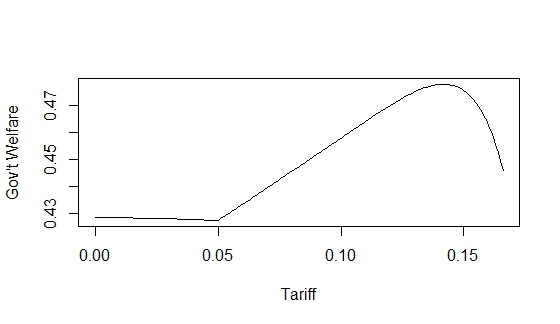
\includegraphics[height=2.75in, width=4.25in]{weight.jpeg}
\end{frame}


\begin{frame}{Comparison to the Literature}
\pause
Others derive non-monotonicity in lobbying effort/tariff 
\pause
\begin{itemize}
	\item Maggi $\&$ Rodriguez-Clare (1998/2007): dynamic firm investment disortions
	\pause
	\item Mitra (2002): lobbies pay investment cost to form
\end{itemize}

\vskip.15in
\pause
Here, I acknowledge the gov't objective function may be fundamentally non-monotonic
\pause
\begin{itemize}[<+->]
	\item Achieve same results with simpler model
	\item Endogenous politics in a wider range of questions
	\item Can have both endogenous / exogenous at the same time $\Rightarrow$ unify the exogenous and endogenous politics literatures
\end{itemize}
\end{frame}


\section{Tariff Caps}
\subsection{Tariff Caps}
\begin{comment}
\begin{frame}{Tariff Caps: Exogenous vs. Endogenous $\ga$}
\pause
Strong binding: an exact tariff commitment
\begin{itemize}
	\pause
	\item Must apply the precise tariff level specified in TA
\end{itemize}

\pause
\vskip.2in
Weak binding: a tariff cap
\begin{itemize}
\pause
	\item Must set tariff at or below specified level 
\end{itemize}

\pause
\vskip.4in
Perfect external enforcement vs. self-enforcement (repeated-game)

\end{frame}



\begin{frame}{Strong Bindings}
Must set tariff at specified level
\pause
\begin{itemize}[<+->]
	\item $\ga$ exogenous (Bagwell $\&$ Staiger 2005): optimal (rigid) strong binding is the tariff that is politically optimal for the expected realization of $\ga$
  \item $\ga$ endogenous: if governments have no inherent bias toward protection, the lobbies exert no effort and are afforded no protection 
\end{itemize}
\end{frame}
\end{comment}

{\begin{frame}{Tariff Caps: Exogenous vs. Endogenous $\ga$}
\pause
Must set tariff at or below specified level (aka weak binding)
\pause
\begin{itemize}[<+->]
	\item $\ga(s)$, i.e. exogenous: Negotiated weak bindings (a) are higher than those gov'ts would choose if they instead negotiated strong bindings and (b) imply that governments with low realizations of $\ga$ set their applied tariffs strictly below the bound level.
		\begin{itemize}
			\item Bagwell $\&$ Staiger 2005 result
		\end{itemize}

	\item $\ga(e)$, i.e. endogenous: Governments will not set applied tariffs strictly below the bound level. They may use the weak tariff binding either to encourage and/or restrain endogenous political pressure.
		\begin{itemize}
			\item Maggi $\&$ Rodriguez-Clare (1998/2007) result
		\end{itemize}

\end{itemize}
\end{frame}


\begin{frame}[label=self]
\frametitle{Tariff Caps with Self Enforcement}
\pause
\begin{itemize}[<+->]
	\item $\ga$ exogenous (Bagwell $\&$ Staiger 2005): if governments patient enough (discount factor $\de$ high enough), optimal externally-enforced weak binding can be self-enforced
  \item $\ga$ endogenous: optimal externally-enforced weak binding may not be self-enforcing
		\begin{itemize}
			\item Problem: lobby is an additional repeated-game player
			\item Lobby's incentive constraint is harder to satisfy as $\de$ increases
		\end{itemize}
	 
\end{itemize}
%\pause
%\hyperlink{repeated<1>}{\beamergotobutton{Repeated Game Intuition}}
\end{frame}




\begin{comment}
\begin{frame}{Highlight: One-Shot Intuition}
\pause
\textbf{Legislature}
\pause
\begin{itemize}
	\item Breaks agreement if median legislator prefers $\btn$ to $\bta$
\end{itemize}

\pause
\vskip.1in
\textbf{Lobby}
\pause
\begin{itemize}[<+->]
	\item Given the $\bta$ it faces, lobby knows what $e_b$ is required to break the agreement
 	\item Lobby pays if $\bm{\pi}(\btn)$ - lobbying costs $> \pi(\bta)$
\end{itemize}

\pause
\vskip.13in
\textbf{Executives}
\pause
\begin{itemize}[<+->]
	\item Set $\bta$ to make paying $e_b$ unprofitable
		\pause
		\begin{itemize}
			\item[$\Rightarrow$] $e_b=0$, agreement remains in force
		\end{itemize}
	\item High tariffs, no lobbying, no trade disruptions
\end{itemize}
\end{frame}
\end{comment}


\begin{frame}[label=repeated]
\frametitle{Repeated Game Intuition}
\pause
Legislature: break agreement if punishment not strong enough
\pause
\begin{itemize}
	\item i.e. if one period of gain from cheater's payoff is greater than T-periods of loss from trade-war
\end{itemize}

\vskip.1in
\pause
Lobby: solve for lowest effort ($\ov{e}_b$) that breaks this constraint
\pause
\begin{itemize}
	\item pay $\ov{e}_b$ if it's less than gain from $T$ periods of trade-war profits
\end{itemize}

\pause
\vskip.1in
Executives: set lowest $\bta$ that makes paying $\ov{e}_b$ unprofitable \textit{and} satisfies legislature's condition
\pause
\begin{itemize}
	\item[$\Rightarrow$] $e_b=0$, agreement remains in force
	\pause
	\item High tariffs, no lobbying, no trade disruptions
\end{itemize}
%\hyperlink{self<1>}{\beamergotobutton{Go Back}}
\end{frame}


\begin{frame}{When the world is more complicated...}
Now suppose $\ga(s,e)$, i.e. political pressure is a result of both endogenous and exogenous forces:
\pause
\vskip.1in
\begin{beamerboxesrounded}[upper=palette tertiary, shadow=true]{Water in the Bindings with $\ga(s,e)$}
  Assume $\ga(s,e) = \ga(s) + \ga(e)$. In order for governments to set applied tariffs strictly below the weak binding, the low shock must be realized \textit{and} the lobby must not have the incentive to `top up' political pressure to the level associated with the binding. 
\end{beamerboxesrounded}

\pause
\begin{itemize}[<+->]
	\item Can happen if gov't mis-judges lobby's incentives
	\item In general, gov't prefers cap because lobby will `fill in' for low shock up to gov's optimal level of $\ga$
\end{itemize}
\end{frame}


\section{Escape Clause}
\subsection{Escape Clause}
\begin{frame}{Escape Clause with Exogenous Politics}

\pause
When $\ga$ is \textit{only} exogenous (Bagwell $\&$ Staiger 2005):

\pause
\begin{itemize}[<+->]
	\item Simple escape clause: add a second (higher) negotiated weak binding
		\begin{itemize}
			\item Escape clause is designed to allow higher applied tariff when realization of $\ga$ is high
		\end{itemize}
	\item Improves political efficiency
	\item Can improve self-enforcement
	\item Incentive compatibility becomes an issue
\end{itemize}
\end{frame}


\begin{frame}{Incentive compatibility}
\pause
Escape clause is meant to allow higher applied tariff when realized $\ga$ is high
\pause
\begin{itemize}[<+->]
	\item $\ga$ is private information
	\item We want truthful revelation, but truth-telling must be in the best interest of each gov't
	\item Gov't can exploit TOT externality by reporting high $\ga$ even when $\ga$ is low
		\begin{itemize}
			\item Only way to prevent this is with some cost of using escape clause
		\end{itemize}
	\end{itemize}
\end{frame}


\begin{frame}{Escape Clause with Endogenous Politics}
When $\ga$ is \textit{only} endogenous:
\pause
\begin{itemize}[<+->]
	\item Benefit of escape clause from exogenous case is gone
	\item Assuming lower binding is set to maximize political welfare, escape clause encourages inefficiently high lobbying effort / protection
	\item Incentive compatibility still an issue, but often not the central one
		\begin{itemize}[<+->]
			\item If lobby's preferred tariff $\geq$ escape clause binding, gov't experiences high $\ga$, no need to lie
		\end{itemize}
  \end{itemize}
	
\vskip.2in
\pause
If $\ga$ is only endogenous, escape clause causes problems, provides no benefits
\end{frame}


\begin{frame}{When the world is more complicated...}
Now suppose political pressure is a result of both endogenous and exogenous forces (i.e. $\ga(s,e)$):
\pause
\begin{itemize}[<+->]
	\item Want escape clause to deal with exogenous shock
	\item But endogenous part $\Rightarrow$ lobbying incentives make it hard to implement escape clause
\end{itemize}

\pause
\vskip.2in
\begin{beamerboxesrounded}[upper=palette tertiary, shadow=true]{Ineffectiveness of Political Criterion for Escape Clause}
  Assume $\ga(s,e) = \ga(s) + \ga(e)$. If an escape clause conditions on $\ga(s,e)$ and $\ga(s^L) < \ga(s^H) < \ga(e^L)$, the lower ``normal'' tariff binding will never be applied.
\end{beamerboxesrounded}
\end{frame}


\begin{frame}{When the world is more complicated... (con't)}
\begin{itemize}[<+->]
	\item To make escape clause work, can't use $\ga$
	\begin{itemize}[<+->]
		\item Need signal of shock that is not influenced by endogenous pressure
	\end{itemize}
	\item Can condition directly on $s$
		\begin{itemize}
			\item This seems to be what the WTO actually \textit{does}
		\end{itemize}
\end{itemize}

\end{frame}


\begin{frame}{An Escape Clause for a Complicated World}
\pause
Assume a WTO-like set up: gov't can choose between $\tau^a$, `escape' tariff $\tau(s)$, or politically-optimal $\tau$ matched to $\ga(s,e)$
\pause
\begin{itemize}[<+->]
	\item Assume $s$ verifiable, so no punishment for $\tau(s)$
	\item Punishment for $\tau(\ga(s,e)) > \tau(s)$
\end{itemize}

\vskip.2in
\pause
Optimal $\tau^a$ may lead government to apply $\tau(\ga(s,e))$
\pause
\begin{itemize}[<+->]
	\item When this happens, it leads to dispute, not valid escape
	\item Otherwise, no extra rent-seeking is encouraged
\end{itemize}

\vskip.2in
\pause
May explain why escape clause has fallen out of use

\end{frame}



%\begin{frame}{Optimal Punishments}
%\begin{beamerboxesrounded}[upper=palette tertiary, shadow=true]{Optimal DSI}
%  In the case of political certainty, if non-trivial cooperation is possible in the presence of a lobby, the optimal punishment scheme is finite when the influence of the lobby on legislative preferences is sufficiently strong $\left(\frac{\partial \gamma}{\partial e} \text{ is sufficiently high} \right)$.
%\end{beamerboxesrounded}
%\end{frame}



\section{Conclusion}
\subsection{}
\begin{comment}
\begin{frame}{Ex-Ante Lobbying}
Without ex-ante: gov't anticipates ex-post lobbying, chooses $\tau^{\text{TA}}$ that maximizes objective function given $e^{\text{EP}}$
  \[
	  \max_\tau W(\ga(e^{\text{EP}}),\tau) + W^*(\tau)
	\]
\pause
When ex-ante lobbying ($e^{\text{EA}}$) is possible, we could have
\pause
  \[
	  \max_\tau W(\ga(e^{\text{EA}}),\tau) + W^*(\tau)
	\]
	but the lobby would now have to pay \textit{twice}.
\end{frame}
\end{comment}

\begin{frame}{Conclusion}
Taking into account endogenous political forces alongside exogenous ones in this simplified modeling framework
\pause
\begin{itemize}[<+->]
		\item demonstrates that TAs can be used to discourage lobbing activity in general
		\item can nest established results and provide new insights
		\item can answer questions about optimal design of trading institutions more fully
			\begin{itemize}
				\item provides additional general explanation for tariff caps
				\item helps explain the structure and enforcement of the WTO Safeguards measure
			\end{itemize}
\end{itemize}

\end{frame}

\begin{frame}{Future Work}
\pause
\begin{itemize}[<+->]
	\item Application of framework to other design questions
	\item Interactions between $\ga(s)$ and $\ga(e)$
	\item Choice between protective measures over time
\end{itemize}

\end{frame}






\end{document}